\documentclass[12pt]{report}
\usepackage[utf8]{inputenc}
\usepackage[russian]{babel}
%\usepackage[14pt]{extsizes}
\usepackage{listings}
\usepackage{graphicx}
\usepackage{amsmath,amsfonts,amssymb,amsthm,mathtools} 
\usepackage{pgfplots}
\usepackage{filecontents}
\usepackage{indentfirst}
\usepackage{eucal}
\usepackage{amsmath}
\usepackage{enumitem}
\usepackage{fixltx2e}
\usepackage{float}

\frenchspacing

\usepackage{indentfirst} % Красная строка


%\usetikzlibrary{datavisualization}
%\usetikzlibrary{datavisualization.formats.functions}

\usepackage{amsmath}


% Для листинга кода:
\lstset{ %
language=caml,                 % выбор языка для подсветки (здесь это С)
basicstyle=\small\sffamily, % размер и начертание шрифта для подсветки кода
numbers=left,               % где поставить нумерацию строк (слева\справа)
numberstyle=\tiny,           % размер шрифта для номеров строк
stepnumber=1,                   % размер шага между двумя номерами строк
numbersep=5pt,                % как далеко отстоят номера строк от подсвечиваемого кода
showspaces=false,            % показывать или нет пробелы специальными отступами
showstringspaces=false,      % показывать или нет пробелы в строках
showtabs=false,             % показывать или нет табуляцию в строках
frame=single,              % рисовать рамку вокруг кода
tabsize=2,                 % размер табуляции по умолчанию равен 2 пробелам
captionpos=t,              % позиция заголовка вверху [t] или внизу [b] 
breaklines=true,           % автоматически переносить строки (да\нет)
breakatwhitespace=false, % переносить строки только если есть пробел
escapeinside={\#*}{*)}   % если нужно добавить комментарии в коде
}

\usepackage[left=2cm,right=2cm, top=2cm,bottom=2cm,bindingoffset=0cm]{geometry}


% plot
\usepackage{pgfplots}
\usepackage{filecontents}
\usetikzlibrary{datavisualization}
\usetikzlibrary{datavisualization.formats.functions}

\graphicspath{ {img/} }


\usepackage{subcaption}

\captionsetup{labelsep=endash}
\captionsetup[figure]{name={Рисунок}}


\begin{document}
	\begin{titlepage}
		\thispagestyle{empty}
		
		\noindent
		\begin{minipage}{0.15\textwidth}
			
\includegraphics[width=\linewidth]{main_logo}
		\end{minipage}
		\noindent
		\begin{minipage}{0.9\textwidth}
			\centering
			\textbf{Министерство науки и высшего образования Российской Федерации}\\
			\textbf{Федеральное государственное бюджетное образовательное учреждение высшего образования}\\
			\textbf{«Московский государственный технический университет имени Н.Э.~Баумана}\\
			\textbf{(национальный исследовательский университет)»}\\
			\textbf{(МГТУ им. Н.Э.~Баумана)}
		\end{minipage}
		
		\noindent
		\rule{18cm}{3pt} %пустая строка
		\newline\newline %пустая строка
		\noindent ФАКУЛЬТЕТ $\underline{\text{«Информатика и системы управления»}}$ \newline\newline
		\noindent КАФЕДРА $\underline{\text{«Программное обеспечение ЭВМ и информационные технологии»}}$\newline\newline\newline\newline\newline
		
		
		\begin{center}
			\noindent\begin{minipage}{1.3\textwidth}\centering
				\Large\textbf{ Домашнее задание №1}\newline
				\textbf{по дисциплине "Анализ алгоритмов"}\newline
                \textbf{по теме "графовые представления"}\newline\newline
			\end{minipage}
		\end{center}
		
		\noindent\textbf{Студент} $\underline{\text{Коняев Е.А}}$\newline\newline
		\noindent\textbf{Группа} $\underline{\text{ИУ7-53Б}}$\newline\newline
		\noindent\textbf{Преподаватели} $\underline{\text{Волкова Л.Л., Строганов Ю.В.}}$\newline\newline
		\noindent\textbf{Дата сдачи отчета}$\underline{\text{~~~~~~~~~~~~~~~~~~~~~~~~~~~}}$\newline\newline
		\noindent\textbf{Оценка (баллы)} $\underline{\text{~~~~~~~~~~~~~~~~~~~~~~~~~~~}}$\newline\newline\newline
		
		\begin{center}
			\vfill
			Москва~---~\the\year~г.
		\end{center}
	\end{titlepage}
	
	\setcounter{page}{2}
	\tableofcontents
	
	\newpage
	\chapter{Выполнение задания}

    \section{Выбор языка программирования и среды разработки}
	
	Для реализации трех алгоритмов сортировок был выбор язык С, так как данный язык является быстродейственным.

	Средой разработки был выбран СLion. Данный выбор обусловлен тем, что данная среда предоставляет возможность разработки приложений под C/C++ и имеет инструменты для отладки кода. 

    \section{Реализации алгоритмов}

    В листинге \ref{lev} представлен итерационный алгоритм нахождения расстояния Левеншетейна. именно данный алгоритм будет рассмотрен в графовом представлении.

	\begin{lstlisting}[label=lev,caption=Листинг итерационного алгоритма нахождения расстояния Левенштейна,language=C]
		int dist_lev(char *str_1, char *str_2, matrix *d, int print_table_flag)
        {
            matrix_t *d = create_matrix(strlen(str_1) + 1, strlen(str_2) + 1);//1
            d->elements[0][0] = 0; //2
            for (size_t i = 1; i < d->rows; ++i) //3
                d->elements[i][0] = i; //4
            for (size_t i = 1; i < d->cols; ++i)  //5
                d->elements[0][i] = i;  //6
            
            for (size_t i = 1; i < d->rows; ++i) //7
                for (size_t j = 1; j < d->cols; ++j) {  //8
                    int offset = 1;  //9
                    if (str_1[i - 1] == str_2[j - 1])  //10
                        offset = 0; //11
                    d->elements[i][j] = get_min(d->elements[i][j - 1] + 1,
                                                d->elements[i - 1][j] + 1,          
                                                d->elements[i - 1][j - 1] + offset); //12 
                }

             if (print_table_flag)  //13
                print_matrix(d);  //14
        
            int res = d->elements[d->rows - 1][d->cols - 1];  //15
            free_matrix(d);    //16
        
            return res;  //17
        }
	\end{lstlisting}

    \section{Графовые представления}

    На рисунках ниже представлен граф операционный, информационный, операционной истории и информационной истории соответсвенно для алгоритма поиска расстояния Левенштейна.

    \begin{figure}[H]
		\centering
		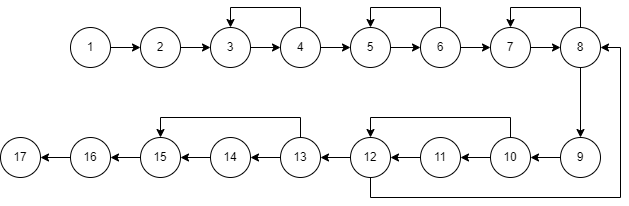
\includegraphics[width=0.9\linewidth]{hw_dia-first.png}
		\caption{Операционный граф}
		\label{fig:ris1}
	\end{figure}

    \begin{figure}[H]
		\centering
		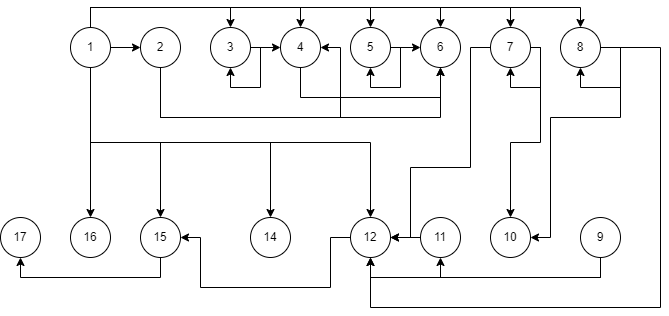
\includegraphics[width=0.9\linewidth]{hw_dia-second.png}
		\caption{Информационный граф}
		\label{fig:ris2}
	\end{figure}

 `  \begin{figure}[H]
		\centering
		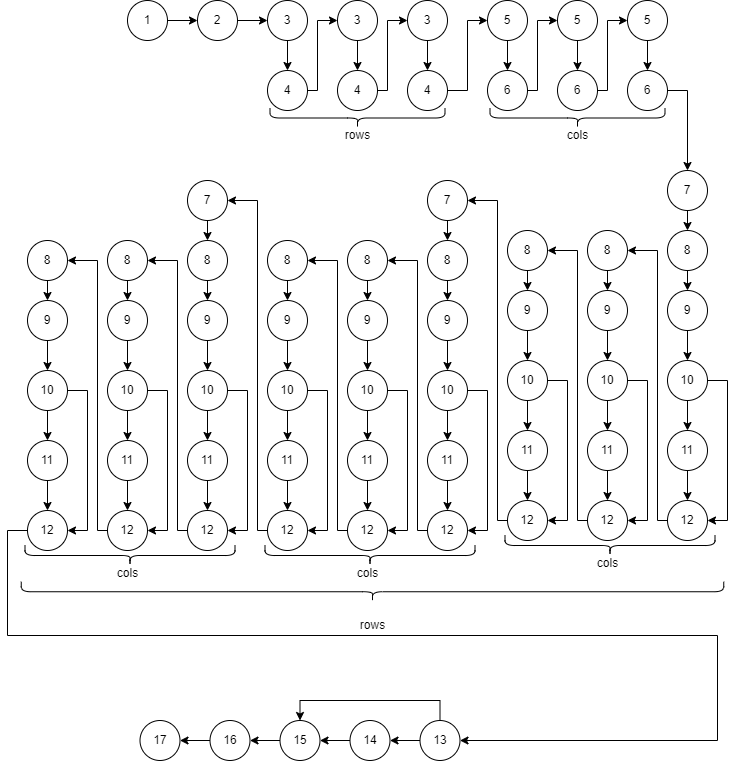
\includegraphics[width=0.9\linewidth]{hw_dia-third.png}
		\caption{Граф операционной истории}
		\label{fig:ris3}
	\end{figure}

    \begin{figure}[H]
		\centering
		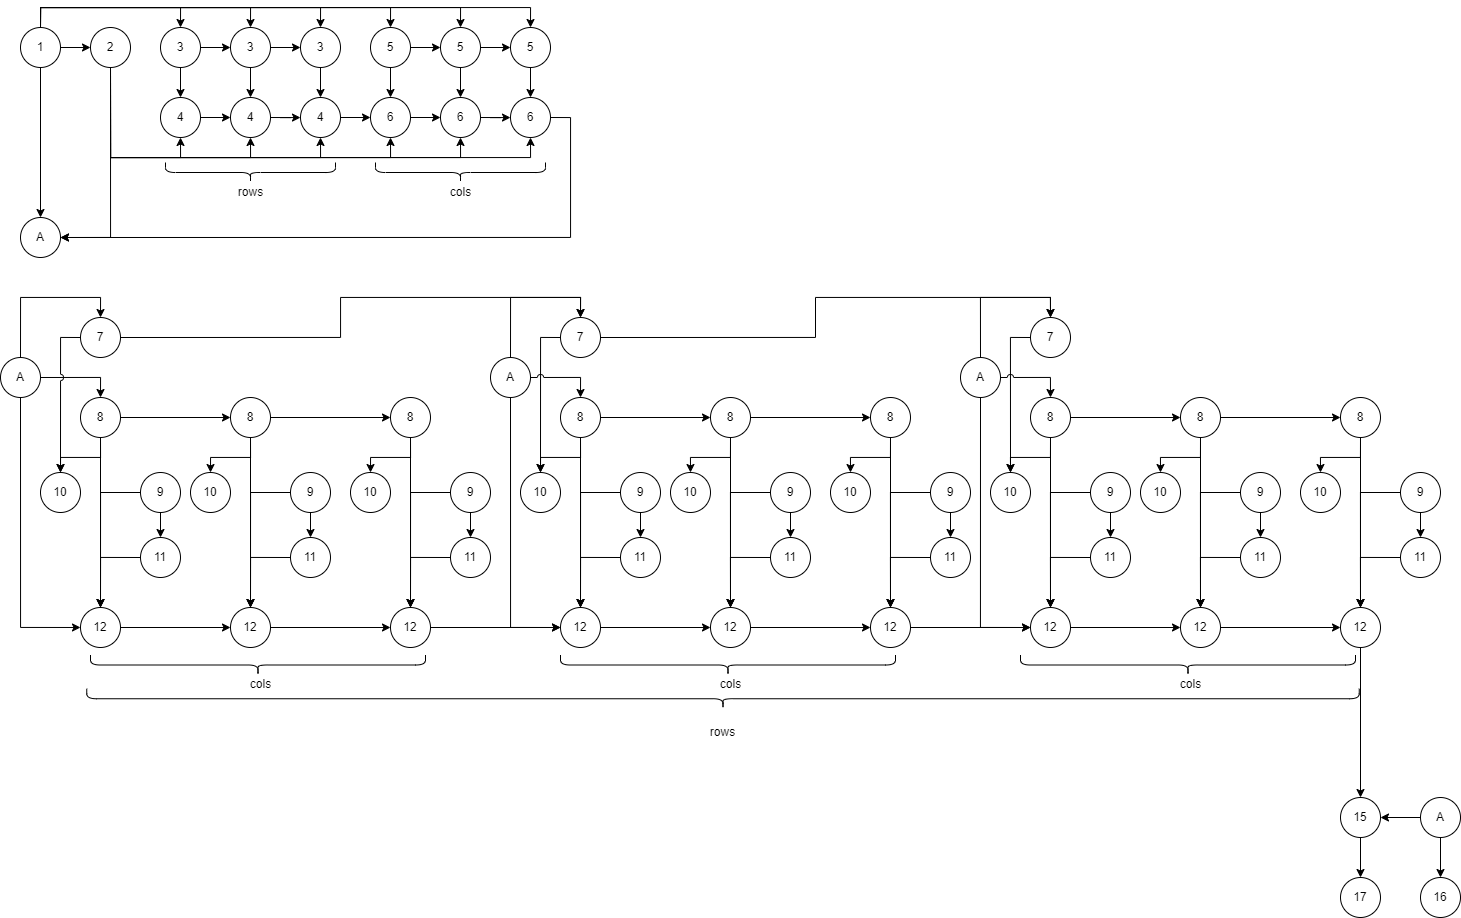
\includegraphics[width=1\linewidth]{hw_dia-fourth.png}
		\caption{Граф информационной истории}
		\label{fig:ris4}
	\end{figure}
	
\addcontentsline{toc}{chapter}{Список использованных источников}

\nocite{*} 

\renewcommand\bibname{Список использованных источников} % переименовать страницу списка литературы
\bibliographystyle{utf8gost705u}  % стилевой файл для оформления по ГОСТу
\bibliography{lib}          % имя библиографической базы (bib-файла)
	
\end{document}
